\documentclass[12pt]{article}
\usepackage[margin=1in]{geometry} 
\usepackage{amsmath,amsthm,amssymb,amsfonts,enumerate,listings,graphicx,epstopdf,siunitx}
\graphicspath{~/Documents/school/fall16/stat586/hw2}
 
\newcommand{\N}{\mathbb{N}}
\newcommand{\Z}{\mathbb{Z}}
 
\newenvironment{problem}[2][Problem]{\begin{trivlist}
\item[\hskip \labelsep {\bfseries #1}\hskip \labelsep {\bfseries #2.}]
  \vspace{1 cm}
}{\end{trivlist}}

\begin{document}
\title{Homework Set 2}
\author{Taylor Bodin}
\maketitle
 
\begin{problem}{2.29} 
\item let $p(m) \equiv E = E_1 \times E_2 \times \dots \times E_m  \rightarrow
  \prod_{i=1}^m n_i$ \\
  \begin{align*}
  p(1) &= E_1 \rightarrow n_1 \\
  p(2) &= E_1 \times E_2 \rightarrow n_1n_2 \\
  \dots \\
  p(k) &= E_1 \times E_2 \times \dots \times E_k \rightarrow \prod_{i=1}^k n_i
  & & \textrm{let the product equal } n_{\textrm{1 to k}} \\
  p(k+1) &= (E_1 \times \dots \times E_k) \times E_{k+1} \rightarrow 
  n_{\textrm{1 to k}}(n_{k+1}) = \prod_{i=1}^{k+1} n_i
  \end{align*}
\end{problem}

\begin{problem}{2.31} 
\item
  \begin{enumerate}[a.]
    \item % A
      \begin{align*}
        {{n}\choose{k}} &= {{n}\choose{n-k}} \\
        \frac{n!}{(n-k)!k!} &= \frac{n!}{(n-k)!(n-(n-k))!} \\
        &= \frac{n!}{(n-k)!(0+k)!} \\
        &= \frac{n!}{(n-k)!k!}
      \end{align*} 
    \item % B
     \begin{align*}
       \binom{n+1}{k+1} &= \binom{n}{k} + \binom{n}{k+1} \\
       \frac{(n+1)!}{(n+1-k-1)!(k+1)!} &= \frac{n!}{k!(n-k)!} + \frac{n!}{(k+1)!(n-k-1)!} \\
       \frac{(n+1)!}{(n-k)!(k+1)!} &= \frac{n!}{k!(n-k-1)!}\left(\frac{1}{n-k} + \frac{1}{k+1}\right) \\
       \frac{(n+1)!}{(n-k)!(k+1)!} &= \frac{n!}{k!(n-k-1)!}\left(\frac{k+1+n-k}{(n-k)(k+1)}\right) \\
       \frac{(n+1)!}{(n-k)!(k+1)!} &= \frac{n!}{k!(n-k-1)!}\left(\frac{n+1}{(n-k)(k+1)}\right) \\
       \frac{(n+1)!}{(n-k)!(k+1)!} &= \frac{(n+1)!}{(n-k)!(k+1)!} 
      \end{align*}
    \item %C
      \begin{align*}
        \sum_{k=0}^n \binom{n}{k} p^k q^{n-k} &= (p+q)^n & & \textrm{let } p = q = 1 \\
        \sum_{k=0}^n \binom{n}{k} 1^k 1^{n-k} &= (1+1)^n \\
        \sum_{k=0}^n \binom{n}{k} &= (2)^n
      \end{align*}
    \item %D
      \begin{align*}
        \sum_{k=0}^n \binom{n}{k} p^k q^{n-k} &= (p+q)^n & & \textrm{let } p = -1, q = 1 \\
        \sum_{k=0}^n \binom{n}{k}(-1)^k 1^{n-k} &= (-1+1)^n \\
        \sum_{k=0}^n \binom{n}{k}(-1)^k &= (0)^n \\
        \sum_{k=0}^n \binom{n}{k}(-1)^k &= 0 
      \end{align*}
    \item %E
      \begin{align*}
        \sum_{k=0}^n \frac{d}{dp}\left( \binom{n}{k} p^k q^{n-k}\right) &= \frac{d}{dp}\left((p+q)^n \right) \\
        \sum_{k=0}^n \binom{n}{k}k p^{k-1} q^{n-k} &= n(p+q)^{n-1} & & \textrm{let } p=q=1 \\
        \sum_{k=0}^n \binom{n}{k}k(1)^{k-1}(1)^{n-k} &= n(1+1)^{n-1} \\
        \sum_{k=0}^n \binom{n}{k}k &= n2^{n-1}
      \end{align*}
    \item %F
       \begin{align*}
        \sum_{k=0}^n \frac{d}{dp}\left( \binom{n}{k} p^k q^{n-k}\right) &= \frac{d}{dp}\left((p+q)^n \right) \\
        \sum_{k=0}^n \binom{n}{k}k p^{k-1} q^{n-k} &= n(p+q)^{n-1} & & \textrm{let } p=-1, q=1 \\
        \sum_{k=0}^n \binom{n}{k}k(-1)^{k-1}(1)^{n-k} &= n(-1+1)^{n-1} \\
        \sum_{k=0}^n \binom{n}{k}k(-1)^{k-1}(-1) &= 0(-1) \\
        \sum_{k=0}^n \binom{n}{k}k(-1)^{k} &= 0 
      \end{align*}
  \end{enumerate}
\end{problem}

\begin{problem}{2.33}
\item
  \begin{enumerate}[a.]
    \item %A
      $P(\textrm{1 Heart}) =  \frac{\binom{13}{1} \binom{39}{12}}{\binom{52}{13}} = \approx \num{8.006e-2}$
    \item %B
      $P(\textrm{7 or more of one suit}) 
      =  \frac{\binom{13}{7} \binom{39}{6}}{\binom{52}{13}} \approx \num{8.817e-3}$
    \item %C
      $P(\textrm{Void of one suit}) 
      = \frac{\binom{13}{0} \binom{39}{13}}{\binom{52}{13}} \approx \num{1.279e-2}$
  \end{enumerate}
\end{problem}

\begin{problem}{2.35}
\item
  \begin{enumerate}[a.]
    \item %A
      $2^n$
    \item %B
      $\frac{\binom{3}{2} \binom{1}{1}}{2^3} = \frac{3}{8}$     
  \end{enumerate}
\end{problem}

\begin{problem}{2.37}
\item
  \begin{enumerate}[a.]
    \item %A
      $N_\textrm{codewords}(n) = \binom{n}{\frac{n}{2}}$, where n is even
    \item %B
      $N_\textrm{codewords}(8) = 70$ but $N_\textrm{codewords}(10) = 252 \therefore N = 10$
  \end{enumerate}
\end{problem}

\begin{problem}{2.39} 
\item
  \begin{enumerate}[a.]
    \item %A
      $\frac{\binom{9}{3}}{2^9} = \frac{21}{128}$
    \item %B
      $\frac{2^9 - \left(\binom{9}{0} + \binom{9}{1} + \binom{9}{2}\right)}{2^9} 
      =  \frac{233}{256} \approx .9102$
    \item %C
      $\frac{2^9 - \left(\binom{9}{0} + \binom{9}{1} + \binom{9}{2} + \binom{9}{8} + \binom{9}{9}\right)}{2^9} 
      =  \frac{57}{64} \approx .8906$
  \end{enumerate}
\end{problem}

\begin{problem}{2.41}
 \item
   \begin{enumerate}[a.]
    \item %A. 
      \begin{align*}
              P(x = 18) &= 2P(A\cap7) + 2P(10\cap8) + 2P(9\cap9) 
              = 2\frac{4}{52}\frac{4}{51} + 2\frac{16}{52}\frac{4}{51} + \frac{4}{52}\frac{3}{51} \\
              P(x = 19) &= 2P(A\cap8) + 2P(10\cap9) 
              = 2\frac{4}{52}\frac{4}{51} + 2\frac{16}{52}\frac{4}{51} \\
              P(x = 20) &= 2P(A\cap9) + P(10\cap10) 
              = 2\frac{4}{52}\frac{4}{51} + 2\frac{16}{52}\frac{15}{51} \\ 
              P(x = 21) &= 2P(A\cap10) 
              = 2\frac{4}{52}\frac{16}{51} \\ 
              P(x \geq 18) &= P(x = 18) + P(x = 19) + P(x = 20) + P(x = 21)
              = \frac{32}{663} +\frac{4}{39} +\frac{40}{663} +\frac{43}{663} 
              = \frac{61}{221}
      \end{align*}
    \item %B
      Using the same method as above:
      \begin{align*}
        P(12) &= \frac{59}{663}\\
        P(13) &= \frac{64}{663}\\
        P(14) &= \frac{59}{663}\\
        P(15) &= \frac{56}{663}\\
        P(16) &= \frac{1}{13}\\
        P(17) &= \frac{16}{221}\\
        P(12 \leq x \geq 17) &= \frac{337}{663}\\
      \end{align*}
  \end{enumerate}
\end{problem}

\begin{problem}{2.43}
\item
  \begin{enumerate}[a.]
    \item %A
      $\binom{52}{5}$
    \item %B
      $P(\textrm{Four Aces}) 
      = \frac{\binom{12}{1}\binom{4}{1}}{\binom{52}{5}}
      = \frac{1}{54145} \approx \num{1.847e-5}$
    \item %C
      $P(\textrm{Four of a Kind}) 
      = \frac{ \binom{13}{1} \binom{12}{1} \binom{4}{1}}{\binom{52}{5}}
      = \frac{1}{4165} \approx \num{2.401e-4}$
  \end{enumerate}
\end{problem}

\begin{problem}{2.45}
\item
  \begin{itemize}
    \item $P(A)$ is the probability of getting a computer from factory A
    \item $P(B)$ is the probability of getting a computer from factory B
    \item $P(D|A)$ is the probability of getting a defective computer given it came from factory A
    \item $P(D|B)$ is the probability of getting a defective computer given it came from factory B
  \end{itemize}
  \begin{align*}
    P(D|A) &= .15 \\
    P(D|B) &= .05 \\
    P(A) &= \frac{1000000}{1000000 + 150000} = \frac{20}{23} \\
    P(B) &= \frac{150000}{1000000 + 150000} = \frac{3}{23} \\
    P(D) &= P(D|A)P(A) + P(D|B)P(B) = .1370
  \end{align*}
\end{problem}

\begin{problem}{2.47}
\item
    \begin{table}[!htpb]
      \centering
      \caption{Known Probabilities for 2.47}
        \label{probs_2_4}
        \begin{tabular}{lll}
          $P(0_{rx}|0_{tx}) = .9$  & $P(0_{rx}|1_{tx}) = .04$ & $P(0_{tx}) = .5$ \\
          $P(1_{rx}|0_{tx}) = .01$ & $P(1_{rx}|1_{tx}) = .8$  & $P(1_{tx}) = .5$ \\
          $P(E_{rx}|0_{tx}) = .09$ & $P(E_{rx}|1_{tx}) = .16$ & $P(E_{tx}) = 0$ 
        \end{tabular}
    \end{table}
  \begin{enumerate}[a.]
    \item %A
            $P(E_{rx}) = P(E_{rx}|0_{tx})P(0_{tx}) + P(E_{rx}|1_{tx})P(1_{tx}) \approx .1250$
    \item %B
      \begin{align*}
        P(0_{tx}|E_{rx}) &= \frac{0_{tx} \cap E_{rx}}{P(E_{rx})} \\
        0_{tx} \cap E_{rx} &= P(E_{rx}|0_{tx})P(0_{tx}) \approx .0450 \\
        P(0_{tx}|E_{rx}) &\approx \frac{.0450}{.1250} \approx .3600
      \end{align*}
    \item %C
      \begin{align*}
        P(P(1_{rx}|0_{tx})\cup P(0_{rx}|1_{tx})) &= P(1_{rx}|0_{tx}) + P(0_{rx}|1_{tx}) & & \textrm{Mutually exclusive} \\
        P(P(1_{rx}|0_{tx})\cup P(0_{rx}|1_{tx})) &= .01 + .04 = .05 
      \end{align*}
  \end{enumerate}
\end{problem}

\begin{problem}{2.49}
\item
  \begin{table}[!htbp]
    \centering
    \begin{tabular}{llllllll}
      Year in School & $P(P)$ & $P(B)$ & $P(G)$ & $P(P|B)$ & $P(P|G)$ & $P(B|P)$ & $P(G|P)$ \\
      2nd grade      & .2774  & .45    & .55    & .25      & .30      & .4054    & .5946    \\
      4th grade      & .37    & .6     & .4     & .35      & .40      & .5676    & .4324    \\
      6th grade      & .5     & .52    & .48    & .5       & .5       & .52      & .48      \\
      8th grade      & .74    & .98    & .02    & .75      & .25      & .65      & .35     
    \end{tabular}
  \end{table}
\end{problem}

\begin{problem}{2.51}
\item
  \begin{enumerate}[a.]
    \item %A
      $P(x=5) = (1-\frac{1}{52})^{5-1} \frac{1}{52} \approx \num{1.779e-2}$
    \item %B
      $P(x\geq5) = (1-\frac{1}{52})^{5-1} \approx .9253$
    \item %C
      \begin{align*}
        P(x=5)
        &= (1-\frac{1}{52})(1-\frac{1}{51})(1-\frac{1}{50})(1-\frac{1}{49})(\frac{1}{48})
        &= \frac{1}{52} \\
        p(x\geq5) 
        &=(1-\frac{1}{52})(1-\frac{1}{51})(1-\frac{1}{50})(1-\frac{1}{49})
        &= \frac{12}{13}
      \end{align*}
  \end{enumerate}
\end{problem}

\begin{problem}{2.53}
\item
  $\frac{1}{2}$
\end{problem}

\begin{problem}{2.55}
\item
  \begin{enumerate}
    \item %A
      \begin{align*}
        P(A\cap \overline{B}) &= P(A)P(\overline{B}) \\
        P(A\cap \overline{B}) &= P(A)(1-P(B)) \\
        \frac{P(A\cap \overline{B})}{P{A}} &= P(\overline{B}) \\ 
        P(\overline{B}|P(A)) &= P(\overline{B}) \\ 
        P(\overline{B}) &= P(\overline{B}) 
      \end{align*}
    \item %B
      \begin{align*}
        P(\overline{A} \cap \overline{B}) &= P(\overline{A})P(\overline{B}) \\
        \frac{P(\overline{A} \cap \overline{B})}{P(\overline{B})} &= P(\overline{A}) \\
        P(\overline{A}|\overline{B}) &= P(\overline{A}) \\
        P(\overline{A}) &= P(\overline{A})
      \end{align*}
  \end{enumerate}
\end{problem}

\begin{problem}{2.57} 
\item
  \begin{enumerate}[a.]
    \item %A
      $P(X=x) = \binom{n}{x}p^x(1-p)^{n-x}$
    \item %B
      \begin{align*}
        (p+q)^n &= \sum_{k=0}^{n} \binom{n}{k}p^kq^{n-k} & & \textrm{let } q = 1-p \\
        (p+1-p)^n &= \sum_{k=0}^{n} \binom{n}{k}p^k(1-p)^{n-k} \\
        1 &= \sum_{k=0}^{n} \binom{n}{k}p^k(1-p)^{n-k} 
    \end{align*}
      \item %C
        The binomial distribution
  \end{enumerate}
\end{problem}

\begin{problem}{2.59} 
  \item %A.
    \begin{figure}[htpb]
      \centering
        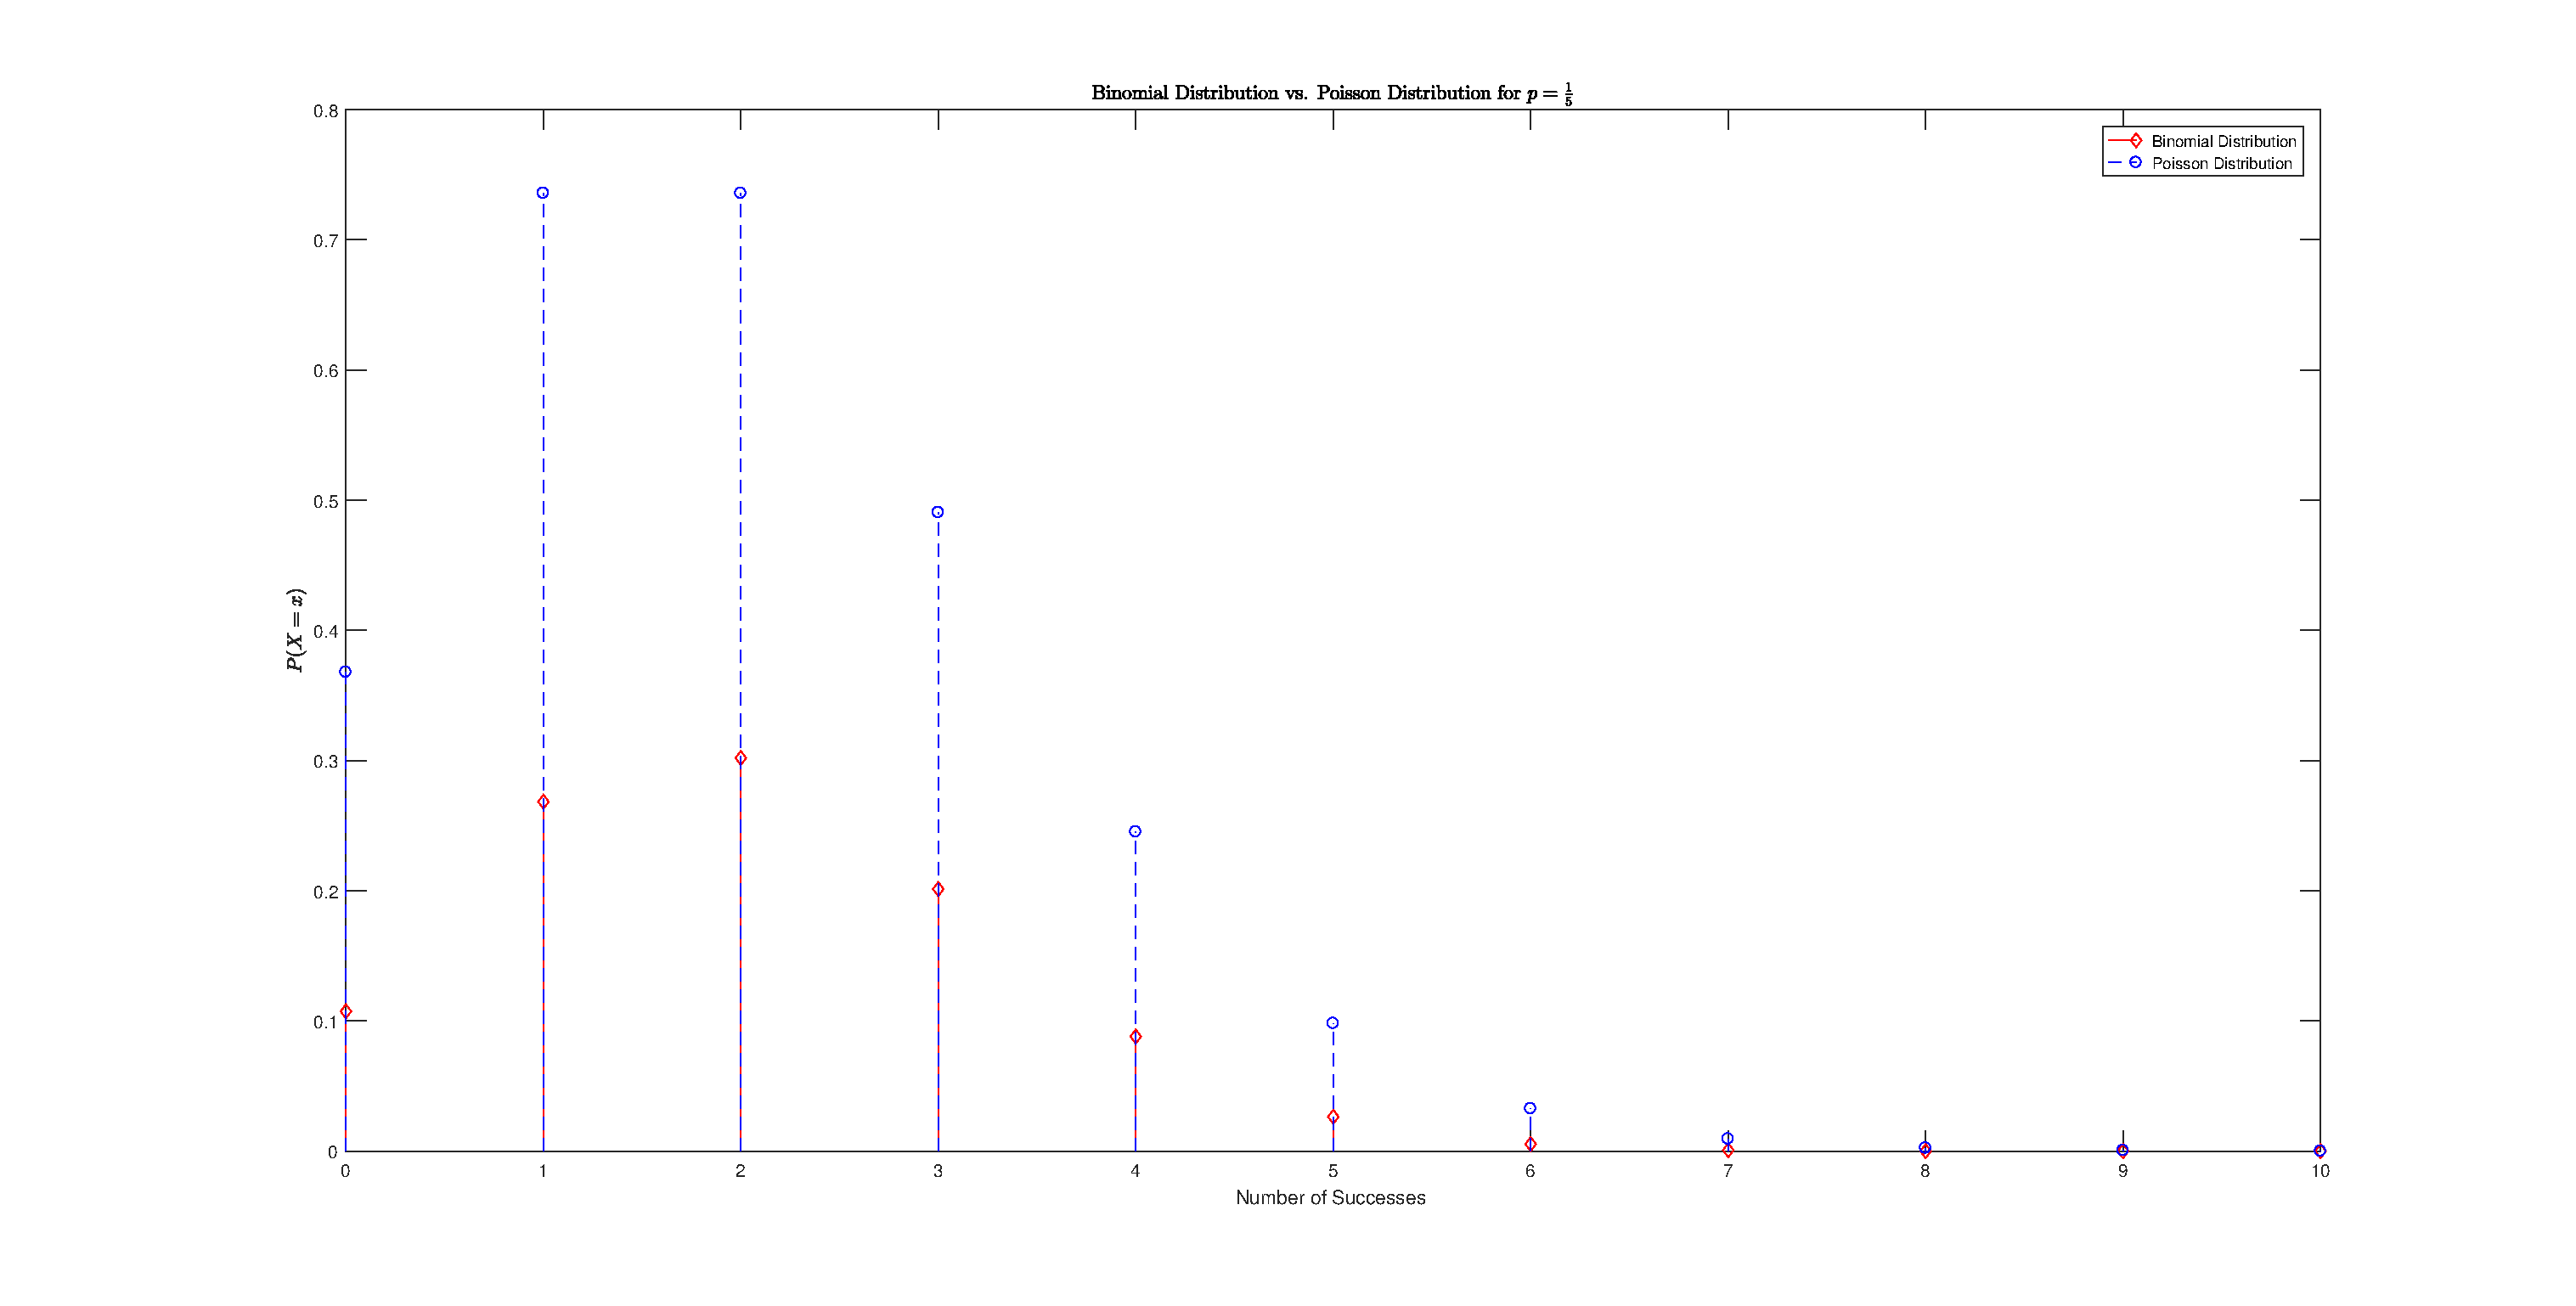
\includegraphics[width=\textwidth,height=\textheight,keepaspectratio]{problem_2_59.eps}
        \caption{Problem 2.59, Binomial vs Poisson}
    \end{figure}
\item %B.
  Figure 1. shows that the Poisson distribution is not a good approximation
  for the binomial distribution for such a small number of experiments and a
  relatively high likelihood of success.
\end{problem} 

\newpage
\begin{problem}{2.61}
\item
  \begin{enumerate}[a.]
    \item %A
      $P(n=1,w=1) = \frac{1}{\binom{50}{6}} = \frac{1}{15890700} \approx \num{6.293e-8}$
    \item %B
      $P(n=\num{6e6},w=4) = \binom{\num{6e6}}{4} (\num{6.293e-8})^4 (1-\num{6.293e-8})^{\num{6e6}-4} \approx \num{5.806e-4}$
    \item %C
      $P(n=\num{6e6},w=0) = \binom{\num{6e6}}{0} (\num{6.293e-8})^0 (1-\num{6.293e-8})^{\num{6e6}-0} \approx .6855$
    \item %D
      $P(n=\num{6e6},w=4) 
      \approx \frac{(\num{6e6}\times\num{6.293e-8})^4}{4!}e^{\num{6e6}\times\num{6.293e-8}} 
      \approx \num{5.807e-4}$ 
    \item %E
      $P(n=\num{6e6},w=0) \approx .6855$
    \item %F
      With the number of trials so high and the probability of success so low,
      the Poisson is a great approximation for the binomial in this case. 
  \end{enumerate}
\end{problem}

\begin{problem}{2.63} 
\item
  \begin{enumerate}[a.]
    \item %A
      $P(n=10,s=1) = \binom{10}{1}(\frac{1}{10})^1(1-\frac{1}{10})^{10-1} \approx .3874$
    \item %B
      $P(n=10,s=0) = \binom{10}{0}(\frac{1}{10})^0(1-\frac{1}{10})^{10-0} \approx .3487$ \\
      $P(n=10,s\geq2) = 1 - (P(n=10,s=0) + P(n=10,s=1)) \approx .2639$
  \end{enumerate}
\end{problem}

\begin{problem}{2.65}
\item
  \begin{enumerate}[a.]
    \item %A
     $P(r) = \frac{18}{18+18+2} \approx .4737$
   \item %B
     $P_N(k) = .5263^{k-1}(.4737)$
   \item %C
     $P_M(k) = \binom{k}{2}(.5263)^{k-2}(.4737)^2$
  \end{enumerate}
\end{problem}

\begin{problem}{2.67}
\item
  \begin{align*}
    P(K = k) &= \sum_{m=0}^k P(M=m)P(N=k-m) \\
    &= \sum_{m=0}^k \left( \frac{\lambda_B^m e^{-\lambda_B}}{m!} \right)
    \left( \frac{\lambda_A^{k-m} e^{-\lambda_A}}{(k-m)!} \right) \\
    &= \sum_{m=0}^k \left( \frac{\lambda_B^m \lambda_A^{k-m} e^{-(\lambda_A+\lambda_B)}}{m!(k-m)!} \right) \\
    &= \frac{e^{-(\lambda_A \lambda_B}}{k!} \sum_{m=0}^{k} \frac{k!}{m!(k-m)!}\lambda_B^m \lambda_A^{k-m} \\
    &= (\lambda_A + \lambda_B)^k \frac{e^{-(\lambda_A + \lambda_B)}}{k!} & & \textrm{by the binomial expansion} \\
    &= \frac{\lambda_C^k e^{-\lambda_C}}{k!} & & \textrm{let } \lambda_A + \lambda_B = \lambda_C
  \end{align*}
\end{problem}

\begin{problem}{2.81} 
\item
  \begin{enumerate}[a.]
    \item %A
      \lstinputlisting{problem_2_81.m}
    \item %B
      \verb|problem_2_81(384,15)| $ = \num{3.3744e26}$ \\
      \verb|nchoosek(384,15)| $ = \num{3.3744e26} $ 
  \end{enumerate}
\end{problem}

\newpage
\begin{problem}{2.83} 
\item
  \begin{enumerate}[a.]
    \item %A
      \lstinputlisting{problem_2_83.m}
    \item %B
            For 2 sets of die:
      \begin{itemize}
        \item $P(\textrm{Offense } = 2, \textrm{Defense }= 0) = 0.2284$
        \item $P(\textrm{Offense } = 1, \textrm{Defense }= 1) = 0.3234$
        \item $P(\textrm{Offense } = 0, \textrm{Defense }= 2) = 0.4483$
      \end{itemize}
     \item %C
            For 3 sets of die:
      \begin{itemize}
        \item $P(\textrm{Offense } = 2, \textrm{Defense }= 0) = 0.2304$
        \item $P(\textrm{Offense } = 1, \textrm{Defense }= 1) = 0.2929$
        \item $P(\textrm{Offense } = 0, \textrm{Defense }= 2) = 0.4767$
      \end{itemize}
  \end{enumerate}
\end{problem}

\end{document}
